\documentclass[conference]{IEEEtran}
\usepackage{cite}
\usepackage{amsmath,amssymb}
\usepackage{booktabs}
\usepackage{graphicx}
\usepackage{url}

\begin{document}

\title{Does Retrieval Make Medical Question Answering More Reliable? A Controlled Evaluation of an Open 7B Language Model on PubMedQA}

\author{
\IEEEauthorblockN{23BCE8207}
\IEEEauthorblockA{VIT-AP University}
\and
\IEEEauthorblockN{23BCE7680}
\IEEEauthorblockA{VIT-AP University}
\and
\IEEEauthorblockN{23BCE7412}
\IEEEauthorblockA{VIT-AP University}
}

\maketitle

\begin{abstract}
Retrieval-augmented generation (RAG) is widely expected to make language models
more dependable for medical question answering. Two assumptions behind this
expectation are rarely tested: that the retriever finds the evidence a question
depends on, and that the model's confidence indicates when it does not. This
paper tests both on the 500-question PubMedQA test set with an open-weight model
(Qwen2.5-7B-Instruct) under four controlled conditions: closed-book answering,
RAG with BM25 or MedCPT retrieval, RAG with the source article withheld, and a
gold-context ceiling. Retrieval success is recorded per question, three leakage
paths are closed, and all settings were fixed on a development split before the
test split was evaluated once. Retrieval raised accuracy from 13.8\% to 36.8\%
(BM25) and 36.0\% (MedCPT), and the gold context reached 43.8\%. On retrieval
misses, RAG was no better than closed-book answering. When the source article
was withheld, the model's confidence did not fall; it rose slightly
(+0.044, 95\% CI [0.030, 0.058]) while its yes/no judgement dropped to chance.
All conditions were dominated by the answer \emph{maybe}, which the prompt
allowed for inconclusive evidence. The results indicate that answer confidence
is not a safe signal for withholding answers when evidence is missing.
\end{abstract}

\begin{IEEEkeywords}
retrieval-augmented generation, medical question answering, calibration,
selective prediction, PubMedQA, large language models
\end{IEEEkeywords}

\section{Introduction}

Medical question answering systems increasingly combine a large language model
(LLM) with a search step over the biomedical literature
\cite{lewis2020rag,xiong2024medrag}. The motivation is intuitive: if the model
reads the relevant study before answering, it should be correct more often and
less likely to assert unsupported conclusions. Most published comparisons of
retrieval-augmented and closed-book answering, however, report accuracy alone
and treat retrieval as a black box. Two questions therefore remain open. When
RAG fails, is the cause a retrieval miss or the model's misuse of the evidence?
And does the model's confidence decrease when the evidence is absent, so that
low-confidence answers could be withheld?

This study examines both questions in a setting where they can be measured
directly. In PubMedQA \cite{jin2019pubmedqa}, each question is derived from one
PubMed article whose abstract settles it, so the document that a perfect
retriever should return is known for every question. The questions, model,
prompt and decoding procedure are held fixed, and only the evidence shown to the
model varies across four conditions (Table~\ref{tab:conditions}). Three research
questions follow:

\begin{itemize}
\item \textbf{RQ1:} What does retrieval contribute (C2 vs.\ C1), in accuracy and
in confident errors?
\item \textbf{RQ2:} What does retrieval failure cost (C3 vs.\ C2, and C2 split
into retrieval hits and misses)?
\item \textbf{RQ3:} Does confidence fall when the key evidence is withheld (C2b
vs.\ C2 on the same questions)?
\end{itemize}

\begin{table}[t]
\centering
\caption{Experimental conditions. Only the evidence changes; question, model,
prompt template and decoding are identical.}
\label{tab:conditions}
\begin{tabular}{@{}lp{3.1cm}p{2.6cm}@{}}
\toprule
ID & Evidence given to the model & Isolates \\
\midrule
C1 & question only & prior knowledge \\
C2 & question + top-$k$ retrieved abstracts & end-to-end RAG \\
C2b & as C2, source article removed & evidence absent \\
C3 & question + source abstract, conclusion removed & perfect retrieval \\
\bottomrule
\end{tabular}
\end{table}

\textbf{Contributions.} The study does not propose a new architecture; its
contribution lies in what is measured and controlled:
\begin{enumerate}
\item A four-condition design that separates retrieval failure from evidence
misuse, with retrieval success of the source article recorded per question.
\item An evidence-withheld condition (C2b) built from a real retriever, which
shows that model confidence does not fall when the key evidence is removed.
\item Explicit controls for three leakage paths in PubMedQA-based retrieval
(answer, title and tuning leakage), including the removal of duplicate
publications of source articles that an identifier-based filter would miss.
\item Reliability measures (confident errors, calibration, risk--coverage) and
a memorisation probe reported alongside correctness, with decision rules fixed
before any model output and a single evaluation of the test split.
\end{enumerate}

\section{Literature Review}

\paragraph*{Retrieval-augmented generation}
RAG conditions a generator on documents returned by a retriever
\cite{lewis2020rag}. Later work lets the model decide when to retrieve and
critique the retrieved passages \cite{asai2024selfrag}. These methods are
evaluated mainly by task accuracy.

\paragraph*{Medical question answering with LLMs}
General-purpose LLMs reach high accuracy on medical benchmarks
\cite{singhal2023medpalm}. MIRAGE/MedRAG \cite{xiong2024medrag} benchmarks
retriever and corpus combinations across five medical QA datasets and introduces
PubMedQA*, in which the gold context is withheld; the C1 and C2 conditions here
build on that setting. MedRGB \cite{ngo2024medrgb} studies robustness to
insufficient or misleading evidence, using constructed contexts and prompted
abstention.

\paragraph*{Retrieval for biomedicine}
BM25 \cite{robertson2009bm25} remains a strong lexical baseline. MedCPT
\cite{jin2023medcpt} is a dense biomedical retriever trained contrastively on
PubMed search logs.

\paragraph*{Confidence, calibration and abstention}
Neural networks are often miscalibrated \cite{guo2017calibration}; LLMs can be
partly calibrated about their own answers \cite{kadavath2022know}. Selective
prediction evaluates confidence by the error rate among the answers a model
chooses to give \cite{geifman2017selective}. Models also use evidence unevenly
across long inputs \cite{liu2024lost}, which motivates varying the number of
retrieved abstracts $k$.

\paragraph*{Memorisation}
LLMs can reproduce training text verbatim \cite{carlini2021extracting}, and
membership in pretraining data can be partly detected \cite{shi2024detecting};
benchmark items published before a model's training cut-off may therefore be
memorised.

\paragraph*{Gap}
Table~\ref{tab:compare} contrasts this study with the closest prior work. To
our knowledge, no prior study combines all four conditions on one benchmark with
one open model while recording whether the source document was retrieved and
reporting calibration alongside correctness.

\begin{table}[t]
\centering
\caption{Comparison with closely related studies (\checkmark: reported;
--: not reported in the cited work, to our knowledge).}
\label{tab:compare}
\setlength{\tabcolsep}{3pt}
\begin{tabular}{@{}lcccc@{}}
\toprule
 & PubMedQA \cite{jin2019pubmedqa} & MedRAG \cite{xiong2024medrag} & MedRGB \cite{ngo2024medrgb} & Ours \\
\midrule
Real retriever & -- & \checkmark & \checkmark & \checkmark \\
Gold-context condition & \checkmark & -- & -- & \checkmark \\
Per-question retrieval success & -- & -- & -- & \checkmark \\
Evidence-withheld condition & -- & -- & \checkmark & \checkmark \\
Measured confidence / calibration & -- & -- & -- & \checkmark \\
Explicit leakage controls & -- & -- & -- & \checkmark \\
\bottomrule
\end{tabular}
\end{table}

\section{Methodology}

\subsection{Dataset and split}
The study uses the 1{,}000 expert-labelled questions of PubMedQA (PQA-L)
\cite{jin2019pubmedqa}: 552 \emph{yes}, 338 \emph{no} and 110 \emph{maybe}. Each
question is its article's title phrased as a question; the context is the
abstract without its conclusion, and the conclusion settles the answer.
\emph{Justification:} PubMedQA provides expert labels, and every question is tied
to a single known source article, which makes per-question retrieval success
measurable. The official PubMedQA test set (500 questions) is used as the test
split and the remaining 500 as a development split; both contain exactly
276/169/55 questions per label. The split is stored with a SHA-256 fingerprint,
and the gold labels of the authors' release and of the HuggingFace copy agree on
all 500 test questions. Answering \emph{yes} to every question gives 55.20\%
accuracy and 0.2371 macro-F1, which serves as a data-loading check and as the
floor.

\subsection{Retrieval corpus and leakage controls}
The corpus contains all PubMedQA abstracts: PQA-L, PQA-U (61{,}249) and PQA-A
(211{,}269), 273{,}518 in total, with no identifier (PMID) shared between
subsets. One abstract forms one document, without chunking, so whether the
source was retrieved has a single answer. Three controls prevent the benchmark's
construction from inflating RAG results:

\begin{enumerate}
\item \textbf{Answer leakage.} Each source article enters the corpus without its
conclusion, exactly as in C3; every other article keeps its full abstract.
Filtering by PMID alone is insufficient: one source study appears under two
further PMIDs with its conclusion intact. Any document sharing at least half (and
at least two) of a source's sentences of eight or more words is therefore
removed; this removes exactly those two copies, while the largest overlap among
retained documents is 12.5\%. A further 75 exact duplicates are removed, leaving
273{,}441 documents.
\item \textbf{Title leakage.} Because each question is its article's title,
titles are never indexed, and section headers are dropped so that the source
cannot be identified by a missing conclusion header.
\item \textbf{Tuning leakage.} All choices were fixed on the development split by
rules recorded before any model output (Section~\ref{sec:prereg}); the test
split was evaluated once.
\end{enumerate}
The corpus build is deterministic; rebuilding it on the GPU machine reproduced
the same SHA-256.

\subsection{Retrievers}
Two retrievers of different kinds are evaluated so that conclusions do not depend
on one retrieval method. \textbf{BM25} \cite{robertson2009bm25} is implemented on
a sparse document--term matrix with Lucene's IDF, $k_1=1.2$, $b=0.75$ (fixed),
Lucene's English stopword list and Porter stemming; on a 5{,}000-document slice it
returns the same top-10 documents as the \texttt{bm25s} library for all 500
development questions, differing only in the order of exactly tied scores.
\textbf{MedCPT} \cite{jin2023medcpt} encodes questions (at most 64 tokens) and
abstracts (at most 512 tokens); documents are ranked by exact inner product.
Because titles are withheld, articles are encoded with an empty title segment.
Of the 273{,}441 abstracts, 8{,}251 (3.0\%) exceed 512 tokens and are truncated;
no question exceeds 64 tokens.

\subsection{Conditions}
For each question the top 100 documents are retrieved once and every condition
is derived from that ranking. C2 uses the top $k$ documents; C2b removes the
source from the ranking and takes the first $k$, which equals retrieving $k{+}1$
and dropping the source, so on a retrieval miss C2b equals C2. C3 contains only
the source with exactly its corpus text. Documents are presented in rank order
and numbered. The prompt template is identical in every condition; only the
block of abstracts changes, and it is absent in C1. The instruction reads:
``Answer the research question with exactly one word: yes, no, or maybe. Use
maybe only when the evidence is inconclusive.''

\subsection{Model, answers and confidence}
The generator is Qwen2.5-7B-Instruct \cite{qwen2024qwen25}, used zero-shot with
fixed weights. \emph{Justification:} an open-weight model fixes the weights across
conditions and allows the analysis to be reproduced, and a 7B model is a
realistic size for local deployment. For each question the model reads the
prompt once. At the answer position, the probabilities of the words \emph{yes},
\emph{no} and \emph{maybe} are read (case variants summed, each a single token),
renormalised over the three, and the largest is taken as the answer. This equals
greedy decoding restricted to the three labels and yields a confidence without
sampling. Before renormalisation, the three labels held 99.98\% of the
probability mass on a 20-question check, so the model answered in the requested
format. The model runs in FP16 on two NVIDIA T4 GPUs.

\subsection{Evaluation metrics and statistics}
\textbf{Correctness:} accuracy, macro-F1, and per-class precision, recall and
F1. Macro-F1 is used because the labels are imbalanced (55/34/11\%).
\textbf{Reliability:} the confident-error rate (share of all questions answered
incorrectly with confidence $\geq\tau$), expected calibration error (ECE) with
ten bins \cite{guo2017calibration}, and the risk--coverage curve with its area
(AURC) \cite{geifman2017selective}, which needs no threshold. \emph{Maybe} is a
gold label meaning the study was inconclusive; answering \emph{maybe} to a
\emph{yes} question is an error, not an abstention. Since answers are labels, no
text is fabricated, and the study measures confident errors rather than claiming
to detect hallucination. \textbf{Statistics:} conditions are compared on the same
questions with exact McNemar tests \cite{mcnemar1947} and 95\% paired bootstrap
intervals \cite{efron1993bootstrap} (10{,}000 resamples, fixed seed). All metrics
are implemented directly and unit-tested against worked examples.

\subsection{Memorisation probe}
Given the title and abstract body followed by ``Conclusion:'', the model
generates greedily; a question counts as memorised if the first eight or more
words reproduce the true conclusion verbatim \cite{carlini2021extracting}.
Paraphrase scores zero by design.

\subsection{Pre-registered decisions and protocol}
\label{sec:prereg}
Before any model output existed, the following were fixed: (i) both retrievers
are reported; (ii) for each retriever, $k\in\{1,3,5,10\}$ is chosen by the highest
development C2 macro-F1, ties to the smaller $k$; (iii) $\tau=0.9$, with 0.8 and
0.95 as sensitivity; (iv) the prompt is changed only if the format check fails.
One script applied these rules, recorded the settings, and only then evaluated
the test split once. The rule selected $k=5$ for BM25 and $k=3$ for MedCPT
(Fig.~\ref{fig:ksweep}).

\subsection{Deviations}
The plan named Llama-3.1-8B-Instruct; because access to its gated weights was not
granted in time, the pre-registered fallback Qwen2.5-7B-Instruct was used with an
identical pipeline. To fit the longest prompts (5{,}602 tokens) in T4 memory,
attention was computed with key/value heads repeated for each query group, which
is mathematically identical to grouped-query attention; on CPU it reproduced the
standard implementation exactly, and all test-split outputs use it. Some
development-split files were computed by an earlier, interrupted run with the
standard implementation; they affect only the choice of $k$. The analysis in
Section~\ref{sec:posthoc} was added after the test results and is labelled as
post hoc.

\section{Results and Discussion}
All results are on the 500 test questions.

\subsection{Retrieval}
The source abstract is among the top five documents for 83.4\% of test questions
with BM25 and 84.8\% with MedCPT (Fig.~\ref{fig:recall}). BM25 ranks the source
first more often (71.6\% vs.\ 64.2\% at $k=1$), whereas MedCPT finds more sources
deeper in the ranking (91.8\% vs.\ 87.6\% at $k=10$; 98.6\% vs.\ 96.6\% at
$k=100$). Retrieval is easier here than for questions posed by clinicians,
because questions are article titles and share vocabulary with their abstracts.
The development macro-F1 varied little with $k$ (0.342--0.357 for BM25,
0.350--0.367 for MedCPT; Fig.~\ref{fig:ksweep}), so adding abstracts beyond a
few brought no clear gain.

\begin{table*}[t]
\centering
\caption{Correctness and reliability per condition on the test split ($n=500$).
Conf.\ err: wrong answers with confidence $\geq 0.9$. Mass: probability on the
three labels before renormalisation. Lower is better for conf.\ err, ECE and
AURC. Majority baseline: 55.2\% accuracy, 0.237 macro-F1.}
\label{tab:main}
\begin{tabular}{lrrrrrrrr}
\toprule
Condition & Acc (\%) & Macro-F1 & R(maybe) (\%) & Conf.\,err (\%) & ECE & AURC & Mean conf. & Mass \\
\midrule
C1 closed-book & 13.8 & 0.107 & 90.9 & 80.4 & 0.836 & 0.879 & 0.974 & 0.999 \\
C2 BM25, $k=5$ & 36.8 & 0.318 & 67.3 & 50.8 & 0.570 & 0.623 & 0.930 & 1.000 \\
C2b BM25, $k=5$ & 15.8 & 0.136 & 89.1 & 77.4 & 0.809 & 0.885 & 0.967 & 1.000 \\
C2 MedCPT, $k=3$ & 36.0 & 0.332 & 63.6 & 51.0 & 0.569 & 0.588 & 0.929 & 1.000 \\
C2b MedCPT, $k=3$ & 15.6 & 0.139 & 85.5 & 76.4 & 0.805 & 0.859 & 0.961 & 1.000 \\
C3 gold context & 43.8 & 0.404 & 60.0 & 43.8 & 0.496 & 0.500 & 0.934 & 1.000 \\
\bottomrule
\end{tabular}
\end{table*}

\begin{table}[t]
\centering
\caption{Per-class precision (P), recall (R) and F1 on the test split.}
\label{tab:perclass}
\setlength{\tabcolsep}{2.5pt}
\begin{tabular}{@{}lrrrrrrrrr@{}}
\toprule
 & \multicolumn{3}{c}{yes} & \multicolumn{3}{c}{no} & \multicolumn{3}{c}{maybe} \\
Cond. & P & R & F1 & P & R & F1 & P & R & F1 \\
\midrule
C1 & 54.5 & 6.5 & .117 & 50.0 & 0.6 & .012 & 10.8 & 90.9 & .192 \\
C2 BM25 & 81.1 & 48.2 & .605 & 77.8 & 8.3 & .150 & 11.6 & 67.3 & .198 \\
C2 MedCPT & 78.9 & 43.5 & .561 & 75.8 & 14.8 & .248 & 11.1 & 63.6 & .189 \\
C3 & 86.5 & 53.3 & .659 & 79.6 & 23.1 & .358 & 11.7 & 60.0 & .196 \\
\bottomrule
\end{tabular}
\end{table}

\subsection{Overall behaviour: the model over-uses \emph{maybe}}
Every condition falls below the 55.2\% majority baseline in accuracy
(Table~\ref{tab:main}). The per-class results (Table~\ref{tab:perclass}) show
why: the model answers \emph{maybe} far more often than the 11\% of questions
that carry that label, with \emph{maybe} recall of 60--91\% but precision of only
11--12\%. Without evidence (C1) it answers \emph{maybe} to 93\% of questions,
with a mean confidence of 0.974. The prompt allowed \emph{maybe} for inconclusive
evidence, and the model applied it whenever evidence was absent or partial. When
it does commit to \emph{yes} or \emph{no}, it is usually right (precision
76--87\% in C2 and C3). The gold-context accuracy of 43.8\% is therefore well
below the 68.1\% and 78.0\% reported for a fine-tuned model and a human
annotator with the same context \cite{jin2019pubmedqa}; the difference is driven
by the \emph{maybe} answers rather than by wrong \emph{yes}/\emph{no} decisions.

\subsection{RQ1: what retrieval contributes}
Retrieval raised accuracy by 23.0 points with BM25 (95\% CI [18.4, 27.6]) and
22.2 points with MedCPT ([17.8, 26.8]), both with McNemar $p<0.001$. Retrieval
changed 140 wrong answers to right ones and 25 right answers to wrong ones (BM25;
134 and 23 for MedCPT). The confident-error rate fell from 80.4\% to 50.8\% and
51.0\%, and AURC fell from 0.879 to 0.623 and 0.588. H1 is supported: retrieval
improves both accuracy and reliability, mainly by moving the model from
\emph{maybe} to correct \emph{yes}/\emph{no} answers.

\subsection{RQ2: what retrieval failure costs}
The gold context added a further 7.0 points over BM25 retrieval ([3.0, 11.0],
$p=0.001$) and 7.8 points over MedCPT ([3.8, 11.8], $p<0.001$). On the 417 BM25
retrieval hits, C2 accuracy was 41.0\%, close to the C3 level; on the 83 misses
it was 15.7\%, against 18.1\% for closed-book answering on the same questions,
with confident-error rates of 80.7\% and 77.1\%. MedCPT showed the same pattern
(101 misses: 15.8\% vs.\ 15.8\% accuracy). On retrieval misses, RAG was therefore
no better than closed-book answering, consistent with H2; the miss subgroups are
small, and these comparisons are descriptive.

\subsection{RQ3: does confidence track the evidence?}
When the source article was withheld (C2b), accuracy fell back to the
closed-book level (15.8\% and 15.6\%), yet mean confidence on the same
retrieval-hit questions rose by 0.044 for BM25 ([0.030, 0.058], $n=417$) and by
0.040 for MedCPT ([0.024, 0.056], $n=399$). H3 is rejected: confidence did not
fall when the key evidence was removed. The risk--coverage curves
(Fig.~\ref{fig:rc}) agree: C2b and C1 have the highest AURC (0.885 and 0.879),
meaning that answering only the most confident questions does not avoid errors
in these conditions. Instead of lowering its confidence, the model switched to
\emph{maybe} with high confidence; under the definitions of this study these are
confident errors, not abstentions. The ranking of conditions is unchanged at
$\tau=0.8$ and $\tau=0.95$ (C1 79.0--82.2\%, C2 46.2--55.4\%, C2b
72.4--81.0\%, C3 38.4--48.2\%).

\begin{figure}[t]
\centering
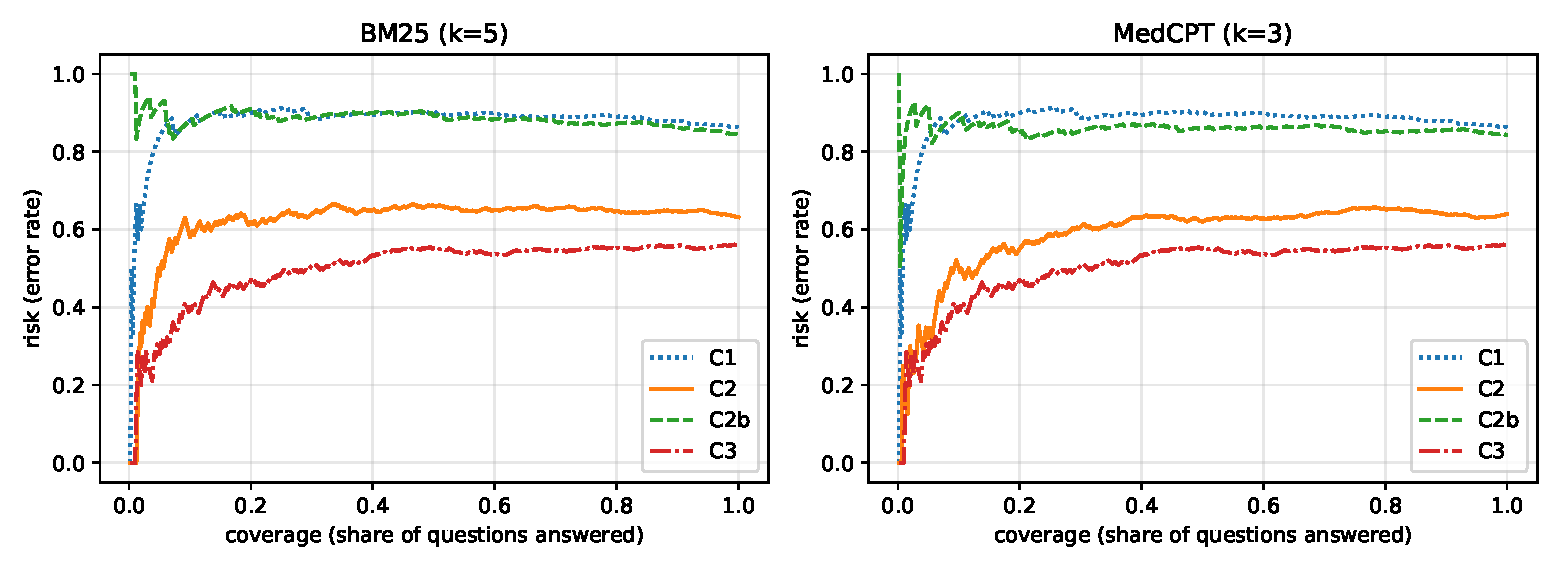
\includegraphics[width=\columnwidth]{fig_risk_coverage.pdf}
\caption{Risk--coverage curves on the test split for BM25 ($k=5$, left) and MedCPT
($k=3$, right). Questions are answered in order of decreasing confidence; the
curve gives the error rate among the answered share. Lower curves indicate a more
useful confidence signal.}
\label{fig:rc}
\end{figure}

\begin{figure}[t]
\centering
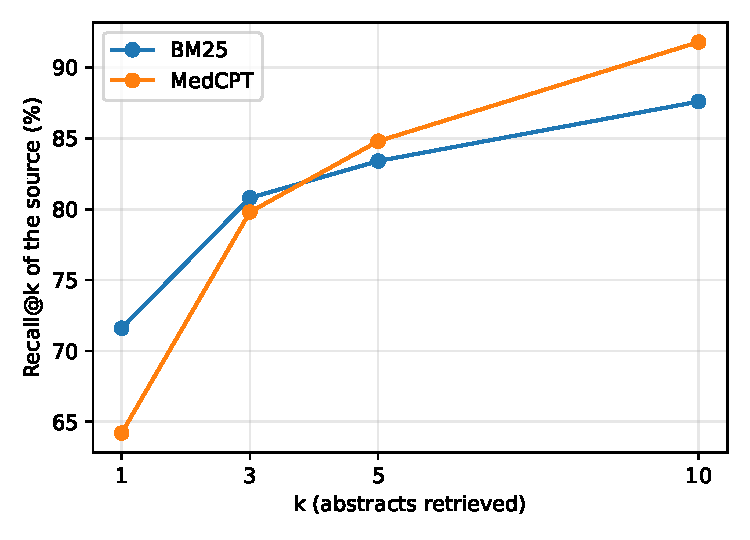
\includegraphics[width=0.85\columnwidth]{fig_recall.pdf}
\caption{Recall@$k$ of the source abstract for BM25 and MedCPT on the test split.}
\label{fig:recall}
\end{figure}

\begin{figure}[t]
\centering
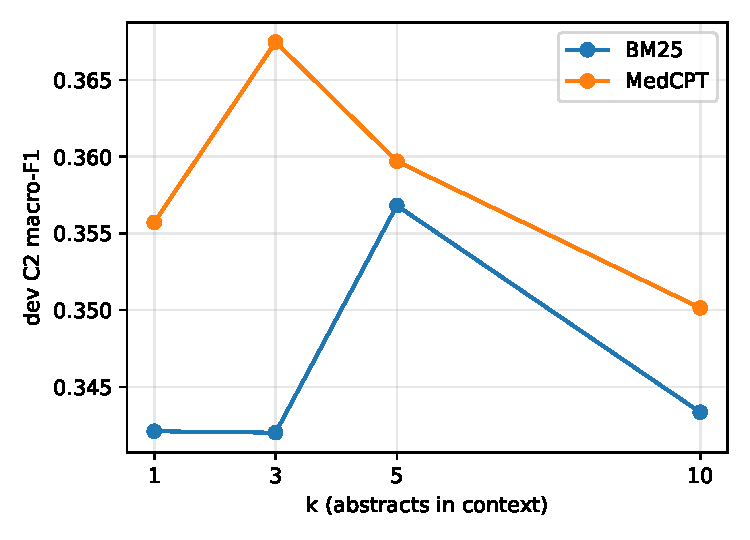
\includegraphics[width=0.85\columnwidth]{fig_k_sweep.pdf}
\caption{Development-split C2 macro-F1 by number of retrieved abstracts $k$. The
pre-registered rule selects the maximum for each retriever ($k=5$ for BM25,
$k=3$ for MedCPT).}
\label{fig:ksweep}
\end{figure}

\subsection{Post hoc analysis: yes/no judgement beneath the \emph{maybe} answers}
\label{sec:posthoc}
Because \emph{maybe} dominated, a supplementary analysis (decided after the test
results and therefore exploratory) asks, for the 445 questions whose gold label
is \emph{yes} or \emph{no}, which of the two the model rates more likely
(Table~\ref{tab:posthoc}). It uses the stored probabilities only. Closed-book,
this judgement is at 58.4\%, below the 62.0\% of always answering \emph{yes}.
Retrieval raises it to 74.6\% (BM25) and 76.4\% (MedCPT), the gold context to
85.4\%, and withholding the source returns it to chance (51.2\% and 50.6\%;
$-$23.4 and $-$25.8 points, $p<10^{-16}$). The model's underlying judgement thus
follows the evidence closely, while its stated confidence does not.

\begin{table}[t]
\centering
\caption{Post hoc: yes-vs-no accuracy on the 445 yes/no test questions, and
paired differences (points, 95\% CI). Always \emph{yes}: 62.0\%.}
\label{tab:posthoc}
\setlength{\tabcolsep}{4pt}
\begin{tabular}{@{}lrr@{}}
\toprule
Condition & \emph{maybe} answers (\%) & yes-vs-no acc.\ (\%) \\
\midrule
C1 & 93.0 & 58.4 \\
C2 BM25 / MedCPT & 63.6 / 63.0 & 74.6 / 76.4 \\
C2b BM25 / MedCPT & 90.4 / 89.0 & 51.2 / 50.6 \\
C3 & 56.2 & 85.4 \\
\midrule
C2$-$C1 (BM25 / MedCPT) & \multicolumn{2}{r}{+16.2 [11.0, 21.6] / +18.0 [13.0, 22.9]} \\
C3$-$C2 (BM25 / MedCPT) & \multicolumn{2}{r}{+10.8 [7.0, 14.6] / +9.0 [5.2, 12.8]} \\
C2b$-$C2 (BM25 / MedCPT) & \multicolumn{2}{r}{$-$23.4 [$-$28.5, $-$18.2] / $-$25.8 [$-$30.8, $-$20.7]} \\
\bottomrule
\end{tabular}
\end{table}

\subsection{Memorisation}
Only 1 of 500 test conclusions was reproduced verbatim, and removing it left the
C2$-$C1 difference unchanged (23.0 and 22.2 points). Verbatim memorisation does
not explain the results; memorised content expressed in other words cannot be
ruled out.

\subsection{Discussion}
Retrieval helped substantially when it worked: it improved accuracy, lowered
confident errors and AURC, and recovered most of the gap to the gold context on
retrieval hits. Its failures were costly in a specific way. On retrieval misses,
the model performed no better than without retrieval, and when the source was
withheld its confidence stayed high while its judgement fell to chance. A system
that withheld low-confidence answers would therefore not have protected users
when evidence was missing. The dominance of \emph{maybe} shows that the answer
behaviour of an instruction-tuned model depends strongly on how an
``inconclusive'' option is phrased, which matters for any benchmark with such a
label.

\subsection{Limitations}
One model and one benchmark are evaluated, so the results may not transfer to
other model families, sizes or datasets. The single prompt allowed \emph{maybe}
for inconclusive evidence, and the model's strong preference for that answer
lowers all accuracies; a different wording may change absolute numbers. PubMedQA
questions are article titles, which makes retrieval easier than for clinicians'
questions. The memorisation probe detects only verbatim recall. MedCPT is used
without titles, and the model runs in FP16. The retrieval-miss subgroups are
small. Nothing in this study supports clinical use.

\section{Conclusion and Future Work}
On PubMedQA with an open 7B model, retrieval raised accuracy by about 23 points
and lowered confident errors, but when retrieval failed the model was no better
than closed-book, and withholding the key evidence did not lower its confidence.
Answer confidence is therefore not a safe abstention signal for missing evidence
in this setting. Future work includes comparing prompt wordings for the
\emph{maybe} option on the development split, extending the four-condition design
to other model families and sizes and to clinicians' questions, and measuring
memorisation beyond verbatim recall.

\section*{Data and Code Availability}
Code, the frozen data split, corpus statistics, the pre-registered settings and
all model outputs are available at
\url{https://github.com/Ashvinj2004/retrieval-reliability-medqa}. A single script
reproduces every reported number from the public data.

\bibliographystyle{IEEEtran}
\bibliography{references}

\end{document}
